
\begin{frame}
  
\frametitle{Outline of this lecture} 

\begin{itemize}

\item Theory of Markov modelling

\item Example: Estimating Markov model transition probabilities from
  individual-level counts of transitions

\item Bayesian inference ideas
  \begin{itemize}
  \item Dirichlet and Multinomial distributions
  \item Advantages of Bayes: including prior information, natural
    quantification of uncertainty (probabilistic sensitivity
    analysis).
  \end{itemize}

\item Implementing Markov models in \texttt{R}

\item Brief discussion of decision modelling more generally, from
  Bayesian perspective
\end{itemize}


\end{frame}


%### New page ############################################################



\frame{
  \frametitle{Markov models in discrete time}

  Assume 
  \begin{itemize}

  \item a set of $S$ ``clinically relevant'' states: exhaustive and mutually exclusive

  \item a discrete time axis, indexed by ``cycles'' or time units $j$

  \item a set of allowed transitions in a diagram of the states
  \end{itemize} 
  
  Arrows connecting two states denote that a person can move
  \begin{itemize}
  \item  from the state at the start of the arrow at time $j$ 
  \item  to the state at the end of the arrow at time $j+1$
  \item Absence of an arrow implies transition is not allowed by model
  \end{itemize}


  \pause
Movements occur according to suitable \alert{\textit{transition probabilities}}
\[ \myblue \bm{\pi}_j = \bm{\pi}_{j-1}\bm\Lambda_j \]
\begin{itemize}
\item $\myblue \bm{\pi}_j$ is the vector of probabilities of occupying each state at time $j$
\item $\myblue \bm\Lambda_j = [\Lambda_{j;s,s'}]$ is the \alert{transition probability matrix} at time $j$: $s,s'$ entry is the probability of moving from state $s$ to state $s'$ at time $j$
\end{itemize}

}

\frame{
\frametitle{Markov models}
\only<1|handout:1>{1.\ Define a structure}
\only<2|handout:2>{2.\ Estimate the transition probabilities from available, relevant data\\Define costs and utilities associated with occupying each state $s$ at each time $j$}
\only<3|handout:3>{3.\ Run the simulation, recording:\\ proportion of people in each state $\rightarrow$ expected costs and effects,\\ at each time:\\ $j=0$}
\only<4|handout:4>{3.\ Run the simulation: $j=1$}
\only<5|handout:5>{3.\ Run the simulation: $j=2$}
\only<6|handout:6>{3.\ Run the simulation: $j=3$}
\only<7|handout:7>{3.\ Run the simulation: $j=J$}
\begin{figure}
\begin{tikzpicture}
\draw(0,1.5) node[align=center,ellipse,draw,fill=none,font=\sffamily\fontsize{9}{10}\selectfont,minimum width=1.8cm,minimum height=.7cm](1){Disease};

\draw(-2.5,0) node[align=center,ellipse,draw,fill=none,font=\sffamily\fontsize{9}{10}\selectfont,minimum width=1.8cm,minimum height=.7cm](2){In health};

\draw(2.5,0) node[align=center,ellipse,draw,fill=none,font=\sffamily\fontsize{9}{10}\selectfont,minimum width=1.8cm,minimum height=.7cm](3){Death};

\draw(0,-1.5) node[align=center,ellipse,draw,fill=none,font=\sffamily\fontsize{9}{10}\selectfont,minimum width=1.8cm,minimum height=.7cm](4){Recovery};

\only<2-|handout:2->{
\draw(-1.4,1.6) node[align=center,fill=none,font=\sffamily\fontsize{9}{10}\selectfont,minimum width=1.8cm,minimum height=.7cm](5){$\lambda_{22}$};

\draw(-4.0,0) node[align=center,fill=none,font=\sffamily\fontsize{9}{10}\selectfont,minimum width=1.8cm,minimum height=.7cm](6){$\lambda_{11}$};

\draw(-1.7,.9) node[align=center,fill=none,font=\sffamily\fontsize{9}{10}\selectfont,minimum width=1.8cm,minimum height=.7cm](7){$\lambda_{12}$};

\draw(1.7,.9) node[align=center,fill=none,font=\sffamily\fontsize{9}{10}\selectfont,minimum width=1.8cm,minimum height=.7cm](8){$\lambda_{24}$};

\draw(-.8,.2) node[align=center,fill=none,font=\sffamily\fontsize{9}{10}\selectfont,minimum width=1.8cm,minimum height=.7cm](9){$\lambda_{14}$};

\draw(4,0) node[align=center,fill=none,font=\sffamily\fontsize{9}{10}\selectfont,minimum width=1.8cm,minimum height=.7cm](10){$\lambda_{44}$};

\draw(.35,-.6) node[align=center,fill=none,font=\sffamily\fontsize{9}{10}\selectfont,minimum width=1.8cm,minimum height=.7cm](11){$\lambda_{23}$};

\draw(-1.7,-.8) node[align=center,fill=none,font=\sffamily\fontsize{9}{10}\selectfont,minimum width=1.8cm,minimum height=.7cm](12){$\lambda_{31}$};

\draw(1.7,-.8) node[align=center,fill=none,font=\sffamily\fontsize{9}{10}\selectfont,minimum width=1.8cm,minimum height=.7cm](13){$\lambda_{34}$};
}

\draw(-2.5,-1.7) node(box_healthy){
\begin{minipage}{0.1\textwidth}
\only<1-2|handout:1-2>{\white
\Gentsroom \Ladiesroom \Ladiesroom \Gentsroom \Gentsroom \Ladiesroom \\
\Ladiesroom \Gentsroom \Gentsroom \Ladiesroom \Ladiesroom \Gentsroom \\
\Gentsroom \Ladiesroom \Ladiesroom \Gentsroom \Gentsroom \Ladiesroom \\
\Ladiesroom \Gentsroom \Ladiesroom \Ladiesroom \Gentsroom \Gentsroom
}
\only<3|handout:3>{\blue
\Gentsroom \Ladiesroom \Ladiesroom \Gentsroom \Gentsroom \Ladiesroom \\
\Ladiesroom \Gentsroom \Gentsroom \Ladiesroom \Ladiesroom \Gentsroom \\
\Gentsroom \Ladiesroom \Ladiesroom \Gentsroom \Gentsroom \Ladiesroom \\
\Ladiesroom \Gentsroom \Ladiesroom \Ladiesroom \Gentsroom \Gentsroom
}
\only<4|handout:4>{\blue
\Gentsroom \Ladiesroom \Ladiesroom \Gentsroom \Gentsroom \Ladiesroom \\
\Ladiesroom \Gentsroom \Gentsroom \Ladiesroom \Ladiesroom \Gentsroom \\
\Gentsroom \Ladiesroom \Ladiesroom \Gentsroom \Gentsroom \Ladiesroom \\
\Gentsroom \white \Ladiesroom \Ladiesroom \Gentsroom \Ladiesroom \Gentsroom
}
\only<5|handout:5>{\blue
\Gentsroom \Ladiesroom \Ladiesroom \Gentsroom \Gentsroom \Ladiesroom \\
\Ladiesroom \Gentsroom \Gentsroom \Ladiesroom \Ladiesroom \Gentsroom \\
\Gentsroom \Ladiesroom \Ladiesroom \Gentsroom \white \Gentsroom \Ladiesroom \\
\Gentsroom \Ladiesroom \Ladiesroom \white\Gentsroom \Ladiesroom \Gentsroom
}
\only<6|handout:6>{\blue
\Gentsroom \Ladiesroom \Ladiesroom \Gentsroom \Gentsroom \Ladiesroom \\
\Ladiesroom \Gentsroom \Gentsroom \Ladiesroom \Ladiesroom \Gentsroom \\
\white \Gentsroom \Ladiesroom \Ladiesroom \Gentsroom \Gentsroom \Ladiesroom \\
\Gentsroom \Ladiesroom \Ladiesroom \white\Gentsroom \Ladiesroom \Gentsroom
}
\only<7|handout:7>{\white
\Gentsroom \Ladiesroom \Ladiesroom \Gentsroom \Gentsroom \Ladiesroom \\
\Ladiesroom \Gentsroom \Gentsroom \Ladiesroom \Ladiesroom \Gentsroom \\
\Gentsroom \Ladiesroom \Ladiesroom \Gentsroom \Gentsroom \Ladiesroom \\
\Gentsroom \Ladiesroom \Ladiesroom \Gentsroom \Ladiesroom \Gentsroom
}
\end{minipage}
};

\draw(3,-1.5) node(box_dead){
\begin{minipage}{0.1\textwidth}
\only<1-3|handout:1-3>{\white
\Gentsroom \Ladiesroom \Ladiesroom \Gentsroom \Gentsroom \Ladiesroom \\
\Ladiesroom \Gentsroom \Gentsroom \Ladiesroom \Ladiesroom \Gentsroom \\
\Gentsroom \Ladiesroom \Ladiesroom \Gentsroom \Gentsroom \Ladiesroom \\
\Ladiesroom \Gentsroom \Ladiesroom \Ladiesroom \Gentsroom \Gentsroom
}
\only<4|handout:4>{
\Gentsroom \Ladiesroom \white \Ladiesroom \Gentsroom \Gentsroom \Ladiesroom \\
\Ladiesroom \Gentsroom \Gentsroom \Ladiesroom \Ladiesroom \Gentsroom \\
\Gentsroom \Ladiesroom \Ladiesroom \Gentsroom \Gentsroom \Ladiesroom \\
\Ladiesroom \Gentsroom \Ladiesroom \Gentsroom
}
\only<5|handout:5>{
\Gentsroom \Ladiesroom \Ladiesroom \Gentsroom \white \Gentsroom \Ladiesroom \\
\Ladiesroom \Gentsroom \Gentsroom \Ladiesroom \Ladiesroom \Gentsroom \\
\Gentsroom \Ladiesroom \Ladiesroom \Gentsroom \Gentsroom \Ladiesroom \\
\Ladiesroom \Gentsroom \Ladiesroom \Gentsroom
}
\only<6|handout:6>{
\Gentsroom \Ladiesroom \Ladiesroom \Gentsroom \Gentsroom \Ladiesroom \\
\Ladiesroom \Gentsroom \Gentsroom \Ladiesroom \white \Ladiesroom \Gentsroom \\
\Gentsroom \Ladiesroom \Ladiesroom \Gentsroom \Gentsroom \Ladiesroom \\
\Ladiesroom \Gentsroom \Ladiesroom \Gentsroom
}
\only<7|handout:7>{
\Gentsroom \Ladiesroom \Ladiesroom \Gentsroom \Gentsroom \Ladiesroom \\
\Ladiesroom \Gentsroom \Gentsroom \Ladiesroom \Ladiesroom \Gentsroom \\
\Gentsroom \Ladiesroom \Ladiesroom \Gentsroom \Gentsroom \Ladiesroom \\
\Ladiesroom \Gentsroom \Ladiesroom \Ladiesroom \Gentsroom \Gentsroom
}
\end{minipage}
};

\draw(0.4,2.1) node(box_disease){
\begin{minipage}{0.1\textwidth}
\only<1-3|handout:1-3>{\white
\Gentsroom \Ladiesroom \Ladiesroom \Gentsroom 
}
\only<4|handout:4>{\red
\Gentsroom \Ladiesroom \Ladiesroom
}
\only<5|handout:5>{\red 
\Gentsroom \Ladiesroom \Gentsroom \Ladiesroom 
}
\only<6|handout:6>{\red 
\Gentsroom \Ladiesroom \Gentsroom 
}
\only<7|handout:7>{\white
\Gentsroom \Ladiesroom \Gentsroom 
}
\end{minipage}
};

\draw(0.4,-2.1) node(box_recovery){
\begin{minipage}{0.1\textwidth}
\only<1-4|handout:1-4>{\white
\Gentsroom \Ladiesroom  
}
\only<5|handout:5>{\green
\Gentsroom 
}
\only<6|handout:6>{\green
\Gentsroom \Gentsroom 
}
\only<7|handout:7>{\white
\Gentsroom \Gentsroom 
}
\end{minipage}
};

\draw [->,>=latex,shorten >=0pt,auto,node distance=3cm,ultra thin] (1.south) -- (4.north);
\draw [->,>=latex,shorten >=0pt,auto,node distance=3cm,ultra thin] (2.40) -- (1.200);
\draw [->,>=latex,shorten >=0pt,auto,node distance=3cm,ultra thin] (2.east) -- (3.west);
\draw [->,>=latex,shorten >=0pt,auto,node distance=3cm,ultra thin] (4.140) -- (2.300);
\draw [->,>=latex,shorten >=0pt,auto,node distance=3cm,ultra thin] (4.40) -- (3.220);
\draw [->,>=latex,shorten >=0pt,auto,node distance=3cm,ultra thin] (1.330) -- (3.140);
\draw [->,>=latex,shorten >=0pt,auto,node distance=3cm,ultra thin] (1) to [out=195, in=160, looseness=3.5] (1);
\draw [->,>=latex,shorten >=0pt,auto,node distance=3cm,ultra thin] (2) to [out=195, in=160, looseness=3.5] (2);
\draw [->,>=latex,shorten >=0pt,auto,node distance=3cm,ultra thin] (3) to [out=345, in=20, looseness=3.5] (3);


\end{tikzpicture}
\end{figure}
}

%### New page ############################################################

\begin{frame}

\frametitle{Markov assumption (discrete time)}

\alert{Markov} models are multi-state models in which next transition
depends only on the current state
\begin{eqnarray*}
&&\Pr(\mbox{state $s'$ at time $j+1 \mid$ history of the process}) = \\
&&\qquad \Pr(\mbox{state $s'$ at time $j+1\mid$ state $s$ at time $j$})
%%%
%%%&&\Pr(\mbox{state} \: j \: \mbox{at \: time} \: t+1\mid\mbox{history \: of \: process})=  \\
%%%&&\qquad \Pr(\mbox{state} \: j \: \mbox{at \: time} \: t+1\mid\mbox{state} \: i \: \mbox{at \: time} \:t)
\end{eqnarray*}

\pause

A Markov model is \alert{time-homogeneous} if this transition probability is the same for all times $j$.  
\begin{itemize}
\item Counterexample: risk of death depends on age.
\end{itemize}

\pause

Non-Markov models can often be made Markov by adding extra states
\begin{itemize}
\item e.g. states \structure{health}$\rightarrow$\structure{disease}$\rightarrow$ \structure{death}
\item suppose risk of death changes with time spent with disease
\item split \structure{disease} into \structure{``early disease''}$\rightarrow$\structure{''late disease''}, with differing risks of death 
\end{itemize}

Remember these models are only approximations to a true process that is usually continuous-time, continuous-state

\end{frame}




\begin{frame}
\addtobeamertemplate{footnote}{}{\vspace{5ex}}
\frametitle{Example: asthma\footnote{Briggs A, Ades AE and Price MJ. \href{http://citeseerx.ist.psu.edu/viewdoc/download?doi=10.1.1.938.9909&rep=rep1&type=pdf}{Medical Decision Making (2003); 23:341-350}\\}}
Five-state model for management of asthma:
\bi
\item STW: Successfully treated week
\item UTW: Unsuccessfully treated week
\item Hex: Hospital-managed exacerbation
\item Pex: Primary care-managed exacerbation
\item TF: Treatment failure - enters a ``usual care'' pattern (absorbing)
\ei

\begin{center}
\rotatebox{0}{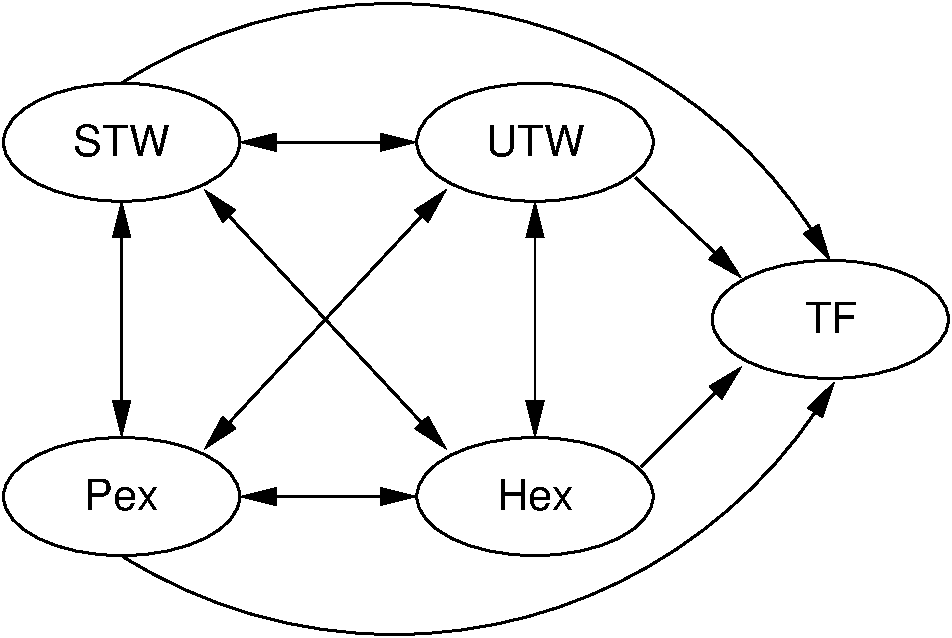
\includegraphics[height=3.5cm]{11.markov-models/figs/5state.pdf}}
\end{center}

\end{frame}


%### New page ############################################################

\begin{frame}

\frametitle{Data}

Estimate the Markov model transition probabilities using individual-level transition data

\bi
\item From a RCT with 2 treatments

\bi
\item SFC: Salmeterol (50$\mu$g) / fluticasone propionate (100$\mu$g) in combination
  \begin{itemize}
  \item new treatment, $t=2$
  \end{itemize}
\item FP: Fluticasone propionate alone (100$\mu$g) 
  \begin{itemize}
  \item existing treatment, $t=1$
  \end{itemize}
  \ei

\item 12 week trial

\item For each arm we count the number of transitions between states from week $j$ to $j+1$

\item From the Markov assumption, these can be considered independent
\ei

\end{frame}

%### New page ############################################################

\begin{frame}

\frametitle{Data}

\begin{center}
\begin{tabular}{l|rrrrr|r} \hline
\multicolumn{7}{c}{SFC} \\ \hline
&\multicolumn{5}{c|}{Number in state at week $j+1$}&Total in state \\
$r_{ss'}$&STW&UTW&Hex&Pex&TF&at week $j$ ($n_s$)\\ \hline
STW & 210 &  60 & 0 & 1 &  1 & 272 \\
UTW &  88 & 641 & 0 & 4 & 13 & 746 \\
Hex &   0 &   0 & 0 & 0 &  0 &   0 \\
Pex &   1 &   0 & 0 & 0 &  1 &   2 \\
TF  &   0 &   0 & 0 & 0 & 81 &  81 \\ \hline \hline
\multicolumn{7}{c}{FP} \\ \hline
STW &  66 &  32 & 0 & 0 &  2 & 100 \\
UTW &  42 & 752 & 0 & 5 & 20 & 819 \\
Hex &   0 &   0 & 0 & 0 &  0 &   0 \\
Pex &   0 &   4 & 0 & 1 &  0 &   5 \\
TF  &   0 &   0 & 0 & 0 &156 & 156 \\ \hline
\end{tabular}
\end{center}

These are summed over all weeks

\end{frame}

%### New page ############################################################

\begin{frame}

\frametitle{Estimating transition probabilities}


 Could estimate $(s,s')$ transition probability by dividing total 
\begin{itemize}
\item number of transitions observed from $s$ to $s'$, by 
\item number of weeks observed in state $s$ 
\end{itemize}

 But can't estimate transition rates out of Hex since nobody went
  into~Hex! \\
 Also very few went into Pex
  \begin{itemize}
  \item estimates / SEs for rates \alert{out of} Pex will be unstable.
  \end{itemize}

 Economic model needs to
  \begin{itemize}
  \item   include possibility of Hex / Pex --
  expensive states! 
\item account for \alert{uncertainty} in the transition
  rates.
  \end{itemize}



  $\rightarrow$ use Bayesian inference
  \begin{itemize}
  \item   -- combine \alert{priors} on
Hex/Pex/other states with data
\item  $\rightarrow$ \alert{posterior}
distribution of transition probabilities.
  \end{itemize}

\end{frame}

%### New page ############################################################

\begin{frame}

\frametitle{Binomial distribution for an event}

Suppose there are two states in the model (\emph{successfully treated
  week} / \emph{treatment failure}).

Out of $n$ people currently under treatment, the following week $r$
people have had treatment failure.

\begin{center}
\input{11.markov-models/figs/2state.pstex_t}
\end{center}

\begin{center}
\begin{tabular}{l||rr}
\hline
Total in STW at $j$ & \multicolumn{2}{c}{Number in state at $j+1$}\\
at week $j$ & STW & TF  \\ \hline
$n$ & $n-r$ & $r$ \\ \hline
\end{tabular}
\end{center}

Beta distribution is a convenient prior for $\lambda$ (conjugacy)

\end{frame}

%### New page ############################################################

%%%%%%\begin{frame}
%%%%%%
%%%%%%\frametitle{Bayesian estimation of binomial model}
%%%%%%
%%%%%%As in drug example, Lectures 1/2. \\ \alert{Likelihood} 
%%%%%%\[
%%%%%%\begin{array}{lllll}
%%%%%%r &\sim &\mbox{Binomial} (\lambda,n)&& \\
%%%%%%\displaystyle p(r\mid\lambda) &=& \frac{n!}{r!(n-r!)}\lambda^r(1-\lambda)^{n-r} &\propto& \lambda^r(1-\lambda)^{n-r}
%%%%%%\end{array}
%%%%%%\]
%%%%%%\alert{Prior}
%%%%%%\[
%%%%%%\begin{array}{lllll}
%%%%%%\lambda &\sim &\mbox{Beta} (a,b)&&  \\
%%%%%%\displaystyle p(\lambda) &=& \frac{\Gamma(a+b)}{\Gamma(a)\Gamma(b)}\lambda^{a-1}(1-\lambda)^{b-1} &\propto& \pi^{a-1}(1-\pi)^{b-1} 
%%%%%%\end{array}
%%%%%%\]
%%%%%%(e.g. prior ignorance: Beta(1,1): uniform (flat) prior on 0--1)
%%%%%%
%%%%%%\alert{Posterior}
%%%%%%\begin{eqnarray}
%%%%%%p(\lambda\mid r) &\propto& \lambda^{a+r-1}(1-\lambda)^{b+n-r-1} \nonumber \\
%%%%%%\lambda\mid r &\sim &\mbox{Beta} (a+r,b+n-r) \nonumber 
%%%%%%\end{eqnarray}
%%%%%%
%%%%%%
%%%%%%\end{frame}
%%%%%%


%### New page ############################################################

\begin{frame}

\frametitle{Multinomial model for several events}

\begin{center}
\input{11.markov-models/figs/5state-1row.pstex_t}
\end{center}

%$\sum \pi_j=1$ 

\begin{center}
\begin{tabular}{ccccc|c} \\ \hline
\multicolumn{5}{c|}{Number in state at $j+1$}&Total in STW at $j$ \\
STW&UTW&Hex&Pex&TF&at week $j$ \\ \hline
$r_1$ & $r_2$ & $r_3$ & $r_4$ &  $r_5$ & $n$ \\ \hline
\end{tabular}
\end{center}


\end{frame}

%### New page ############################################################

\begin{frame}

\frametitle{Bayesian estimation of multinomial model}
%\vspace{-1.5cm}

\textbf{Likelihood}
\myblue
\[
\begin{array}{lllll}
r_1, \ldots, r_5  &\sim &\multicolumn{3}{l}{\mbox{Multinomial} (\lambda_1, \ldots, \lambda_5,n)} \\
p(\bm r\mid\bm\lambda) &=& \frac{n!}{r_1! \cdots r_5!}\lambda_1^{r_1} \ldots \lambda_5^{r_5} &\propto& \lambda_1^{r_1} \ldots \lambda_5^{r_5} \\
\sum \lambda_s &=& 1
\end{array}
\]

\black  
\textbf{Prior distribution for five transition probabilities}
\myblue
\[
\begin{array}{lllll}
(\lambda_1,\ldots,\lambda_5) &\sim &\mbox{Dirichlet} (a_1,\ldots,a_5)&&  \\
p(\lambda_1,\ldots,\lambda_5) &=& \frac{\Gamma(a_1+\cdots+a_5)}{\Gamma(a_1)\cdots\Gamma(a_5)}\lambda_1^{(a_1-1)}\cdots\lambda_5^{(a_5-1)} &\propto& \lambda_1^{(a_1-1)}\cdots\lambda_5^{(a_5-1)} 
\end{array}
\] 

\black  
\textbf{Posterior distribution}
\myblue
\begin{eqnarray}
p(\bm\lambda\mid \bm r) &\propto& \lambda_1^{(a_1+r_1-1)}\cdots\lambda_5^{(a_5+r_5-1)} \nonumber \\
\bm\lambda &\sim & \mbox{Dirichlet} (a_1+r_1,\ldots, a_5+r_5)\nonumber 
\end{eqnarray}

\end{frame}


\begin{frame}

\frametitle{Dirichlet prior distribution}

\begin{itemize}
\item General prior for a set of numbers that add up to 1. 
\item[] $(p_1, \ldots, p_S) \sim \mbox{Dirichlet}(a_1, \ldots, a_S)$
\begin{itemize}
\item $a_s$ proportional to \alert{expected} probability $p_s$ of outcome $s$
\item scale of the $a_s$ indicates prior \alert{precision} of $(p_1, \ldots, p_S)$
\end{itemize}

\vspace{10pt}
\item \textbf{NB}: $\mbox{Dirichlet} (1,\ldots, 1)$ is a flat prior.
\item Given a sample size $\sum a_s$, $a_s$ is your prior expectation for the number
of patients you would expect in each state $s$
\end{itemize}

\end{frame}


\begin{frame}[fragile]

  \frametitle{Simulating from a Dirichlet in \R}

  However the Dirichlet posterior is known here. 

  We can simulate directly from a known Dirichlet distribution in \R by
  exploiting that a Dirichlet random vector is a function of Gamma
  random variables:
  \begin{itemize}
  \item Simulate $Z_s \sim \mbox{Gamma}(a_s, 1)$ for $s=1, \ldots, S$. Then
  \item $(Z_1, \ldots,  Z_S) / \sum_{i=1}^S Z_i \sim \mbox{Dirichlet} (a_1,\ldots,a_S)$
  \end{itemize}

  \pause
  
  For example, to simulate 1000 draws from a Dirichlet(1,1,1,1):

  {\footnotesize \olive
\begin{verbatim}
a <- c(1, 1, 1, 1)
dir_rand <- matrix(nrow=1000, ncol=4)
for (i in 1:4)
    dir_rand[,i] <- rgamma(1000, a[i], 1)
dir_rand <- dir_rand / rowSums(dir_rand)
\end{verbatim}
  }

  \pause
  
  Or functions to simulate directly from the Dirichlet are provided in several \R add-on packages available from CRAN, e.g.

  {\footnotesize \olive
\begin{verbatim}
install.packages("VGAM") # if not already installed
library(VGAM)
dir_rand <- rdiric(1000, a)
\end{verbatim}
}
  
\end{frame}



\begin{frame}

\frametitle{Estimated transition probabilities versus observed data}
% \vspace{-2cm}

After obtaining the posterior Dirichet distributions
{\footnotesize

\begin{tabular}{l|rrrrr||rrrrr} \\ \hline
&\multicolumn{5}{c||}{\alert{Raw transition counts}} & \multicolumn{5}{c}{\alert{Bayesian posterior mean}} \\ \hline
    \textbf{To:}&STW&UTW&Hex&Pex&TF  &STW&UTW&Hex&Pex&TF\\ \hline
\textbf{From:}&\multicolumn{10}{c}{SFC} \\ \hline
 STW & 210 &  60 & 0 & 1 &  1 & 0.76 & 0.22 & 0.004 & 0.01 & 0.01  \\  
 UTW &  88 & 641 & 0 & 4 & 13 & 0.12 & 0.85 & 0.001 & 0.01 & 0.02  \\  
 Hex &   0 &   0 & 0 & 0 &  0 & 0.20 & 0.20 & 0.20 & 0.20 & 0.20   \\  
 Pex &   1 &   0 & 0 & 0 &  1 & 0.29 & 0.14 & 0.14 & 0.14 & 0.28   \\  
 TF  &   0 &   0 & 0 & 0 & 81 &   0 &   0 & 0 & 0 & 1              \\ 
 \hline
 &\multicolumn{10}{c}{FP} \\ \hline
 STW &  66 &  32 & 0 & 0 &  2 & 0.64 & 0.31 & 0.01 & 0.01 & 0.03   \\  
 UTW &  42 & 752 & 0 & 5 & 20 & 0.05 & 0.91 & 0.001 & 0.00 & 0.03  \\  
 Hex &   0 &   0 & 0 & 0 &  0 & 0.20 & 0.20 & 0.20 & 0.20 & 0.20   \\  
 Pex &   0 &   4 & 0 & 1 &  0 & 0.10 & 0.50 & 0.10 & 0.20 & 0.10   \\  
 TF  &   0 &   0 & 0 & 0 &156 &  0 &   0 & 0 & 0 & 1               \\ 
 \hline 
\end{tabular}
}

\vfill \small
Information from the prior has been combined with the data

\end{frame}


%### New page ############################################################

%%%%\begin{frame}
%%%%\frametitle{Cost effectiveness modelling}
%%%%
%%%%\begin{center}
%%%%\begin{overpic}[height=6.5cm]{10.markov-models/figs/5state-animation-1.png}
%%%%\only<2->{\put(0,0){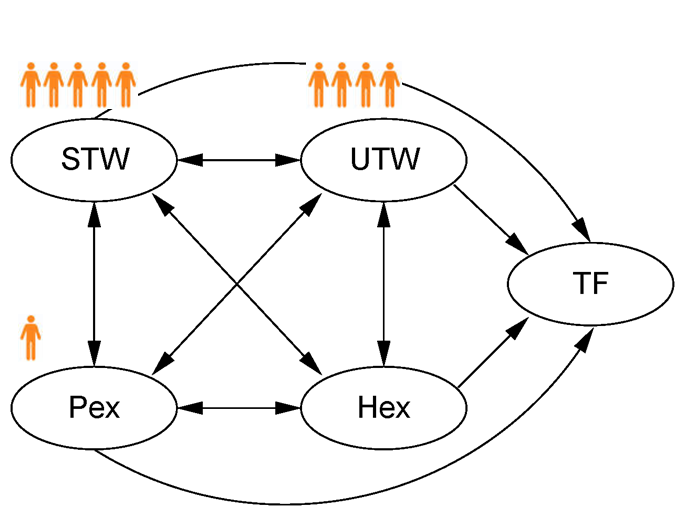
\includegraphics[height=6.5cm]{10.markov-models/figs/5state-animation-2.png}}}
%%%%\only<3->{\put(0,0){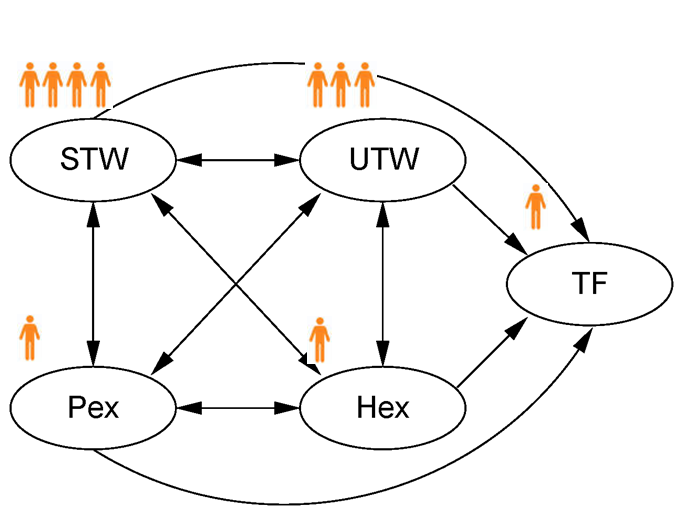
\includegraphics[height=6.5cm]{10.markov-models/figs/5state-animation-3.png}}}
%%%%\only<4->{\put(0,0){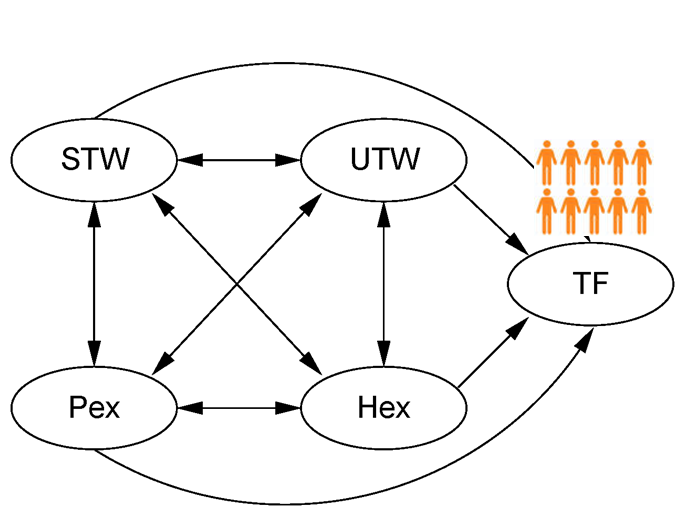
\includegraphics[height=6.5cm]{10.markov-models/figs/5state-animation-4.png}}}
%%%%\end{overpic}
%%%%\end{center}
%%%%
%%%%\end{frame}

%### New page ############################################################

\begin{frame}
\frametitle{Cost-effectiveness modelling}

Calculate \alert{expected costs} and \alert{expected benefits} of each
treatment over the long term:

\begin{itemize}

\item \alert{Cohort simulation:} Estimate proportion of population in each state at each successive time
  (from Markov \emph{transition probabilities})
  \begin{itemize}
  \item at the start, everyone in ``base'' state (e.g. just received treatment) 
  \item usually in the long run, everyone will be in the ``absorbing'' state (e.g.~death)
  \end{itemize}
\vspace{10pt}

\item Assign cost and benefit to each state in model 
\vspace{10pt}

\item Accumulate expected cost and benefit over times

\end{itemize}

\vfill \footnotesize \textbf{NB}: Check BMHE 5.4 + practical!
  
\end{frame}

\frame{
\frametitle{Discounting}
\begin{itemize}

\item Costs and outcomes can occur at different times with respect to when the intervention is implemented

  \begin{itemize}

  \item Society tends to value benefits that arrive closer to the present time more than those that are achievable later in the future

  \end{itemize}

\item \alert{Discounting} accounts for differential timing by reducing the value of costs \& effects in the future

  \begin{itemize}

\item Particularly relevant for economic evaluation spanning over a time horizon $>$ 1 year (e.g. Markov models)
\end{itemize}

\pause

\item If cost at some future time $j$ is $c_{tj}$, then \alert{discounted} cost is $c_{tj}/(1+d)^j$.

\item Discount rate $d$: NICE suggest 3.5\% for costs and outcomes

\item \textbf{Present Value} of intervention (treatment) $t$ over a time horizon $J$ is \color{myblue}
\begin{eqnarray*}
\text{PV}^c_t = \sum_{j=0}^{J}\frac{c_{tj}}{(1+d)^j} \qquad \text{PV}^e_t = \sum_{j=0}^{J}\frac{e_{tj}}{(1+d)^j}
\end{eqnarray*} \color{black}
(for \color{blue}costs $c$ \color{black}and \color{red}clinical benefits $e$\color{black}, respectively)
\end{itemize}
}

%### New page ############################################################

\begin{frame}

\frametitle{Simulating prevalences of states over time}

\begin{itemize}
\item $\pi_{js}$ is the \textbf{expected proportion} of patients in state $s$ at time $j$
\item $\lambda_{ss'}$ is the probability of going from state $s$ to state $s'$ in one time step
\item Thus \myblue 
$$\pi_{j+1,s}=\pi_{j1}\lambda_{1s}+\cdots+\pi_{jS}\lambda_{Ss}$$
\black 
which we can write in matrix form as \myblue
\[
\begin{array}{rcl}
(\pi_{j+1,1},\ldots,\pi_{j+1,S})&=&(\pi_{j,1},\ldots,\pi_{j,S})
\left(
\begin{array}{ccc}
\lambda_{11} & \ldots & \lambda_{1S} \\
\vdots & \ddots & \vdots \\
\lambda_{S1} & \ldots & \lambda_{SS} 
\end{array}
\right) \nonumber \\
\bm{\pi}_{j+1}&=&\bm{\pi}_j \bm\Lambda
\end{array}
\]
\black 
\item \textbf{NB}: $\bm\Lambda$ may depend on time $j$

\pause

\item Instead of calculating \textbf{expected} proportions $\pi_{js}$, could
  simulate the \textbf{absolute number} $m_{js}$ of patients in a
  cohort of size $M$, in state $s$, at time $j$.
  \begin{itemize}
  \item may help to illustrate what model is doing, though decision is generally based on \alert{expected} cost (average cost for an infinite population)
  \end{itemize}
  
\end{itemize}





\end{frame}


\begin{frame}[fragile]
\frametitle{Coding this in \texttt{R} \small{(see BMHE 5.4)}}

Markov cost-effectiveness models can be implemented straightforwardly in \R. 

{\footnotesize \olive
\begin{verbatim}
  pi_sfc <- pi_fp <- array(dim = c(n.sims, # number of PSA samples 
                              S,    # number of states 
                              J+1)) # number of times 
  for (i in 1:n_sims){                # Assumes only 1 patient
      pi_sfc[i,,1] <- c(1,0,0,0,0)    #  initially in the state 
      pi_fp[i,,1] <- c(1,0,0,0,0)     #  'In health'
  }

  for (i in 1:n.sims) {
      for (j in 2:(J+1)){
          for (s in 1:S){
              pi_sfc[i,s,j] <- sum(pi_sfc[i,,j-1]*lambda_sfc[i,,s])
              pi_fp[i,s,j] <- sum(pi_fp[i,,j-1]*lambda_fp[i,,s])
          }
      }
  }
\end{verbatim}
  

}

Many different ways to write code like this: see the questions sheet / solutions for another way. \\

See also \texttt{heemod}, an \R package designed for health economic modelling \url{https://CRAN.R-project.org/package=heemod}

\end{frame}

%### New page ############################################################

\begin{frame}

\frametitle{Costs and utilities}
\begin{itemize}
\item Assign a cost to each state for each treatment
\begin{center}
\begin{tabular}{l|rrrrr} \\ \hline
&\multicolumn{5}{c}{Cost per week (\pounds)} \\
Treatment&STW&UTW&Hex&Pex&TF\\ \hline
SFC & 7.96 & 7.96 & 1821.17 & 100.79 & TF cost (j)\\
FP  & 2.38 & 2.38 & 1815.58 &  95.21 & TF cost (j)\\ \hline
\end{tabular}
\end{center}

\vspace{7pt}
\item In this example, assume the expected cost for week $j$ in SFC group is
$$\myblue \pi_{j1}\times\mathrm{cost}_{(SFC,1)}+\cdots + \pi_{j4}\times\mathrm{cost}_{(SFC,4)}+ \pi_{j5}\times\mbox{TF\:cost}(j) \vspace{-6pt}  \black$$
\begin{itemize}
\item $\displaystyle \myblue \mbox{TF\:cost}(j) = \pi_{j1}\mathrm{cost}_{(FP,1)}+ \cdots + \pi_{j4} \mathrm{cost}_{(FP,4)}$ $=$ average cost over states, weighted by probability of occupying state, under old treatment
\end{itemize}
\vspace{7pt}
\item Utility measure is the number of weeks in the successfully controlled state
\end{itemize}
\end{frame}

%### New page ############################################################

\begin{frame}[fragile]

\frametitle{Expected costs and effects from a Markov model in \R}
%\vspace{-1.5cm}

Combining probabilities of state occupancy (\texttt{pi\_sfc}) with state-specific costs and utilities, for SFC treatment group (with similar code for FP group)

{\footnotesize \olive
\begin{verbatim}
state_costs_sfc <- c(STW=7.96, UTW=7.96, Hex=1821.17, Pex=100.79, TF=NA)
state_util_sfc <- c(1, 0, 0, 0, 0)
cost_sfc <- eff_sfc <- numeric(nsim)

## Loop over PSA samples
for (i in 1:nsim){
    cts <- ets <- numeric(J)

    ## Loop over times j
    for (j in 1:J){
        state_costs_sfc["TF"] <- state_costs_sfc[1:4] %*% pi_sfc[i,1:3,j]
        # costs for time j, averaged over states
        cts[j] <- sum(pi_sfc[i,,j] * state_costs_sfc) 
        # effects for time j, averaged over states
        ets[j] <- sum(pi_sfc[i,,j] * state_util_sfc)  
    }
    # expected costs and effects summed over all times, and averaged over states
    # for PSA sample i
    cost_sfc[i] <- sum(cts) 
    eff_sfc[i] <- sum(ets) 
}
\end{verbatim}
}



\end{frame}

%### New page ############################################################

\begin{frame}[fragile]

\frametitle{Summary: Bayesian health economic model}
% \vspace{-1.5cm}

At each iteration of ``probabilistic sensitivity analysis'', for each arm 

\bi
\item \noindent\textbf{Step 1}: 
\bi
\item draw a realization of the transition probabilities $\bm\Lambda$ from their posterior distribution 
\item define starting state and set time $j=1$
\ei

\vspace{5pt}\pause
\item \noindent\textbf{Step 2}: Markov model
\bi
\item Set time $j = j+1$
\item find prevalence of states $\pi_j$ at this time
\item combine $\pi_j$ with state-specific cost and utility to calculate expected cost and utility at this time
\item repeat step 2 up to time horizon $j = J(=13$ in this case) 
\ei

\vspace{5pt}\pause
\item \noindent\textbf{Step 3}: Cost-effectiveness
\bi
\item calculate expected \alert{costs} 
\item calculate expected \alert{effects} (here, proportion of time spent in STW)
  \ei
  summed over times
  \ei

  Gives a sample from the \textbf{posterior distribution} of expected costs and effects:
  vectors \verb+cost_sfc, eff_sfc, cost_fp, eff_fp+ in R code
\end{frame}


%### New page ############################################################

\begin{frame}

\frametitle{Results}
%\vspace{-1.5cm}

Sample from \alert{joint posterior distribution} of costs and effects
for each treatment gives, e.g. 
\begin{itemize}
\item \alert{incremental cost-effectiveness ratio} = mean cost difference / mean benefit difference
\item ``cost-effectiveness plane''
\item incremental net benefit (with CI)
\item cost-effectiveness acceptability curve
\end{itemize}

\begin{center}
\rotatebox{0}{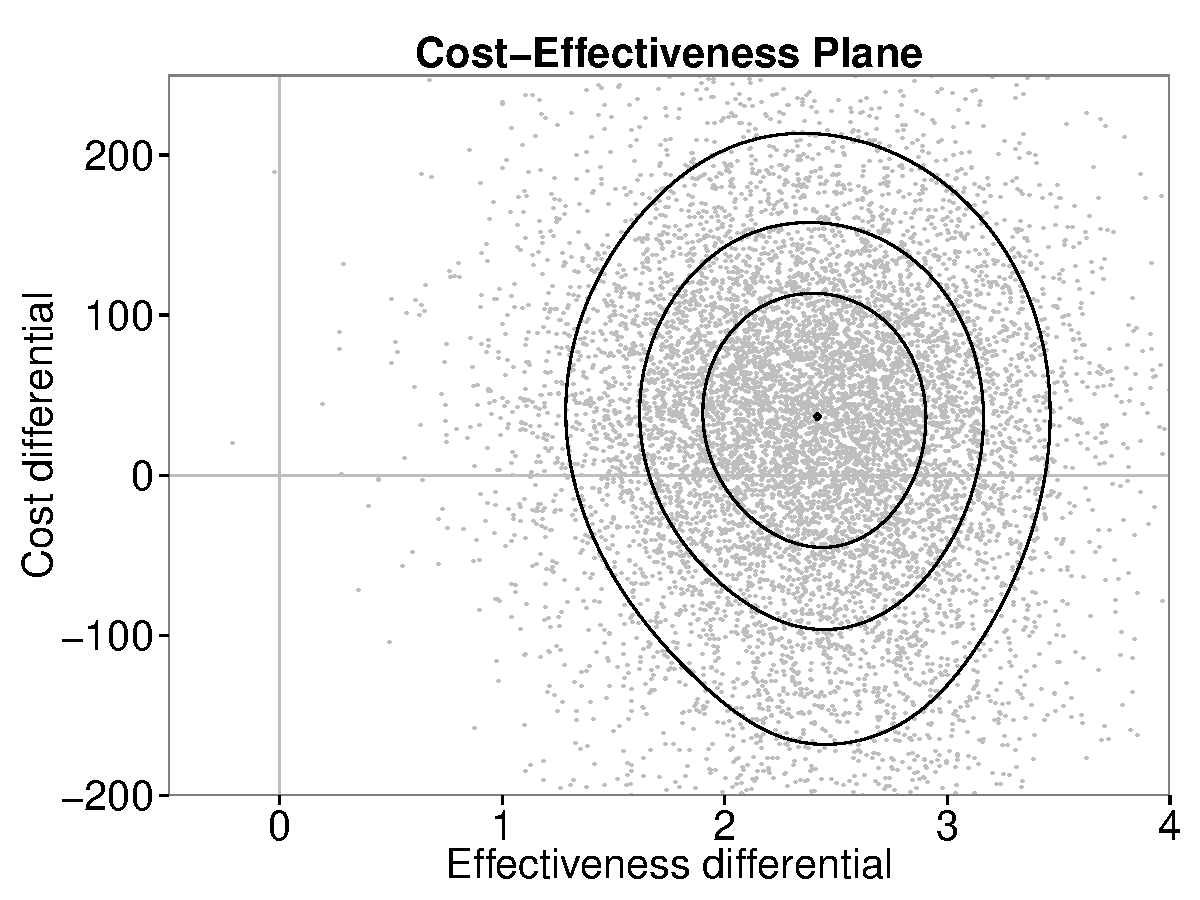
\includegraphics[height=4cm]{11.markov-models/figs/markov5-contour.pdf}}
\rotatebox{0}{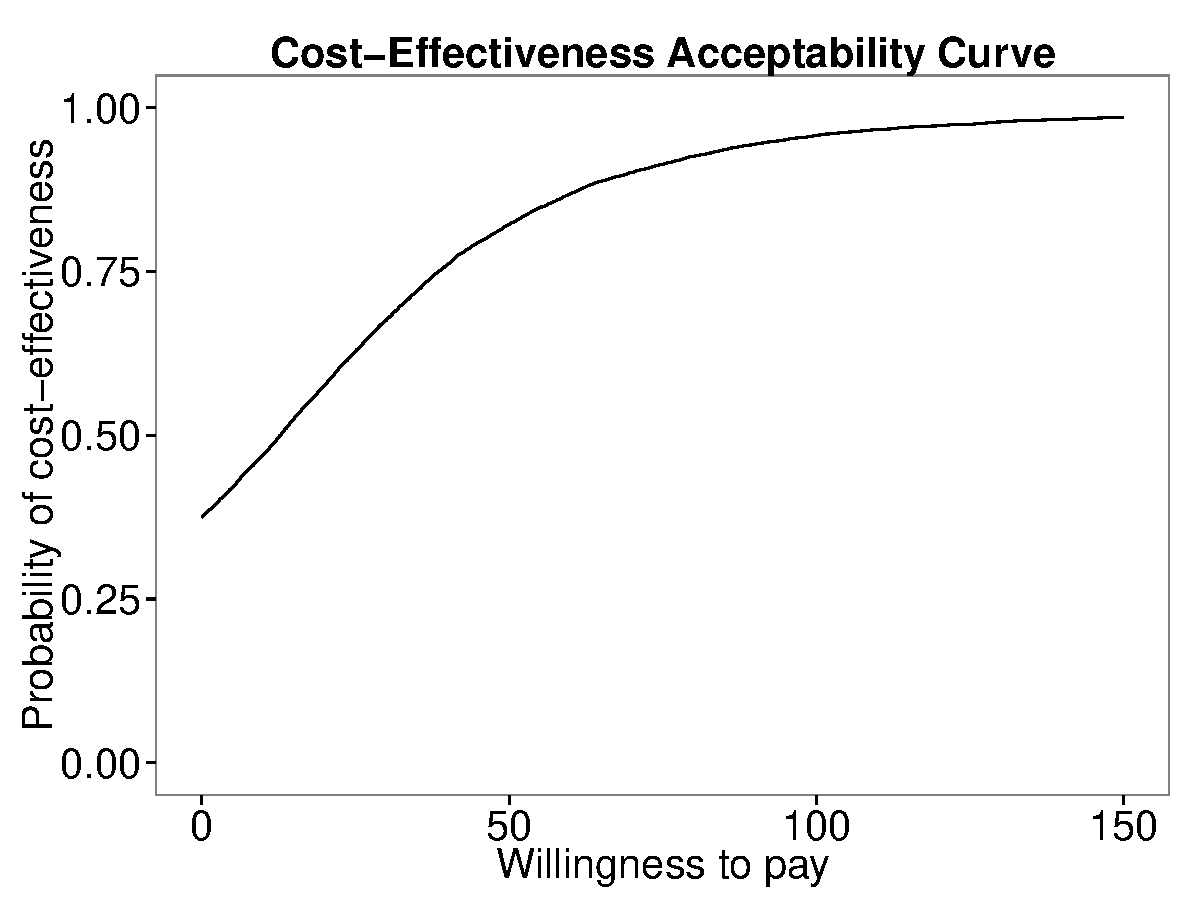
\includegraphics[height=4cm]{11.markov-models/figs//markov5-ceac.pdf}}
\end{center}

\end{frame}


\begin{frame}
  \frametitle{Bayesian decision modelling more generally}

  Example given here was simple
  \begin{itemize}
  \item Markov model with all transition probabilities estimated from
    individual-level transition count data.
  \end{itemize}

  Many more complicated examples, e.g. 

  \begin{itemize}

  \item Transition probabilities for baseline disease progression
    estimated from published data

  \item Treatment effects estimated from RCTs /
    (network-)meta-analysis $\rightarrow$ transition probabilities for
    treated groups

  \item Combinations of individual-level and published aggregate data$\ldots$

  \end{itemize}

  Examples in:
  \begin{itemize}
  \item   \bmhe,
  \item   \emph{Evidence Synthesis for Decision Making in Healthcare},
  \item   \url{http://nicedsu.org.uk/technical-support-documents/}
  \end{itemize}
 
\end{frame}

